\documentclass{article}

\usepackage{amsmath}
\usepackage{graphicx}
\usepackage{courier}
\usepackage{multicol}
\usepackage{microtype} %required to fix courier linebreaking issues
\usepackage{hyperref} % make references into links
\hypersetup{colorlinks=true, linkcolor=blue} %make them pretty links
\usepackage[all]{hypcap} %make them link to the right place

\begin{document}
	\title{AC290r.1: Influence Maximization Problem}
	\author{Stephen Carr and Charles Liu}
	\date{\today}
	\maketitle
	
	\section{Introduction}
	
	\subsection{Goal and Motivation}
	
	From a marketing perspective, social networking sites provide a large number of users with personal and persuasive information regarding products. With limited resources, one would want to know how to reach advertisement to the most number of people in this personalized manner. This problem can be reduced to a graph, where each user is a node and each relationship between users is represented by an edge with some weight to indicate the strength of their relationship. Which user, or set of users, has the ability to spread your product to the greatest number of potential customers?
	
	\subsection{Data set}
	
	The user network of the online restaurant reviewing site Yelp is used in this study. Each account represents the node, and the edges are to be generated by looking at which accounts posted reviews of the same restaurant within a certain time period of one another. This information (the user, their total number of reviews, and how many reviews they have written within 1 month of another user) was pulled from the Yelp site, turned into a library format, and then imported into a python development environment using network x. For most of the prototyping of a solution, a subset of the North Carolina network was taken, which consisted of 240 nodes and ???? edges.
	
	\subsection{Independent Cascade, $I(s)$}
	
	We start with a set of nodes $s = \{n_1,n_2,...,n_k\}$ and wish to find the number of nodes which are activated through our probabilistic network of influence. So for each node $n$ in our original set $s$, we look at all nodes connected to $n$ by an edge and use the beta distribution to determine if the connected node $n_c$ activates (we ignore $n_c$ if it is already activated). The beta distribution $\boldsymbol{B}$ is given by:
	\begin{equation}
	\boxed{
			\int_{-\infty}^{\infty} \frac{dx}{\boldsymbol{B}(\alpha,\beta)}x^{\alpha-1}(1-x)^{\beta - 1} = 1
		}
	\end{equation}
	Where $\beta$ is taken to be the number of reviews node $n_c$ has written within one month of node $n$ writing a review of the same restaurant, and $\alpha$ is taken to be the number of reviews $n_c$ has written. A uniform distribution is taken between $0$ and $1$ and if its value is less than $\boldsymbol{B}(\alpha,\beta)$ then $n_c$ activates and we repeat the same process for neighbors of $n_c$. This recursive process continues until either all nodes are activated or no activated nodes are left in the loop. The number of nodes activated is called $I(s)$.
	
	
	\section{Stochasticity}
	
	\subsection{Averaged Trial Function, $f_N(s)$}
	
	Since each step of the independent cascade is a random sampling of the beta distribution, there is no guarantee that two different measurements of $I(s)$ will be the same, or even "close" to one another, as seen in \ref{fig:Inf_1000}. 
	
	\begin{figure}[h!]
		\centering
		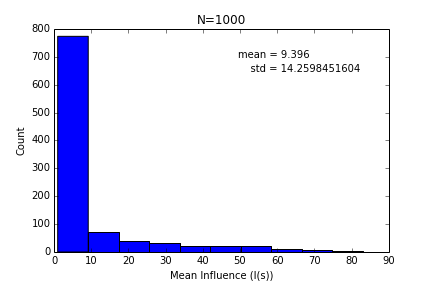
\includegraphics[width=100mm]{N1000_influence.png}
		\caption{Histogram of values $I(s)$ over 1000 iterations for a fixed node in the 240 North Carolina subgraph.}
		\label{fig:Inf_1000}
	\end{figure}
	
	Because of this, we must define a new measurement of a node's influence, namely its mean over $N$ samples:
		\begin{equation}
		\boxed{
			f_N(s) = \frac{1}{N}\sum_1^N I(s)
		}
		\end{equation}
		
		
		
	\subsection{Properties of $f_N(s)$}
	Obviously we cannot take $N$ arbitrarily large, so we must understand how $f_N$'s properties vary with $N$. Taking a 240 node subset of North Carolina, we obtain the following relationship between $N$ and the standard deviation of $f_N$ in \ref{fig:lambda}.
	
		\begin{figure}[h!]
			\centering
			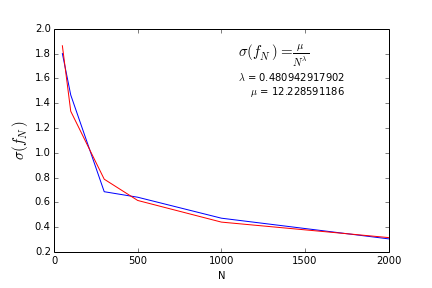
\includegraphics[width=100mm]{lambda_regression.png}
			\caption{Fitted regression for the standard deviation of $f_N(s)$. This was with 100 trials for each N value. The blue line is the simulation, while the red line is the fitted relationship.}
			\label{fig:lambda}
		\end{figure}
			
	
	\subsection{Greedy Algorithm}
		Although this problem is inherently non-linear in its parameters (the starting set of nodes), we can try to solve it in a linear way. This is called the "Greedy Algorithm":
		Given nodes $s_i = \{n_1, n_2,..., n_i\}$, check every remaining node to find node ${n_{i+1}}$ that maximizes $f(s_{i+1})$ where $s_{i+1} =  \{n_1, n_2, ..., n_i, n_{i+1}\}$.
		
		The greedy algorithm of order $k$ looks for $s_k$ satisfying the above condition. For $k = 3$ on our 240 node North Carolina subset we found variation in the maximal $I(s)$ (run and attach $\Delta$ figure).
	
		So even in this simple solution implementation, we see a wide degree of randomness in our answer.	
		
	\section{Implementation}
		
	Markov Chain Monte Carlo (MCMC)
		
	What is Simulated Annealing?
		
		\begin{equation}
		\boxed{
			P(s_1,s_2) = e^\frac{-\Delta E}{T}, \Delta E(f(s_2),f(s_1))
		}
		\end{equation}
		
		The simplest form for $\Delta E$ is $f(s_1) - f(s_2)$. In this case, if $f(s_2) > f(s_1)$ we take $s_2$ with probability 1, otherwise there is a chance of taking $s_2$ even though its estimated influence is less than our current state. This gives us an additional parameter to control our MCMC method: the "Temperature" $T$ controls how likely we are to take a step away from a maximum. So when we are not "near" a local maximum, a high $T$ allows us to sweep the parameter space quickly, but as we near a solution we take a low $T$ to make the MCMC very sensitive to small changes in $f_N(s)$.
	
	Address uncertainties in the optimization.
	
	
	
\end{document}